\svnkwsave{$RepoFile: lyapunov/dailyBlog.tex $}
\svnidlong {$HeadURL$}
{$LastChangedDate$}
{$LastChangedRevision$} {$LastChangedBy$}
\svnid{$Id$}


\chapter{\KS}
\label{sect:LyapKS}

% PC 2009-09-12: (b) generated by siminos/figSrc/gnu/lyapSpec.gnu
\begin{figure}
 (a)~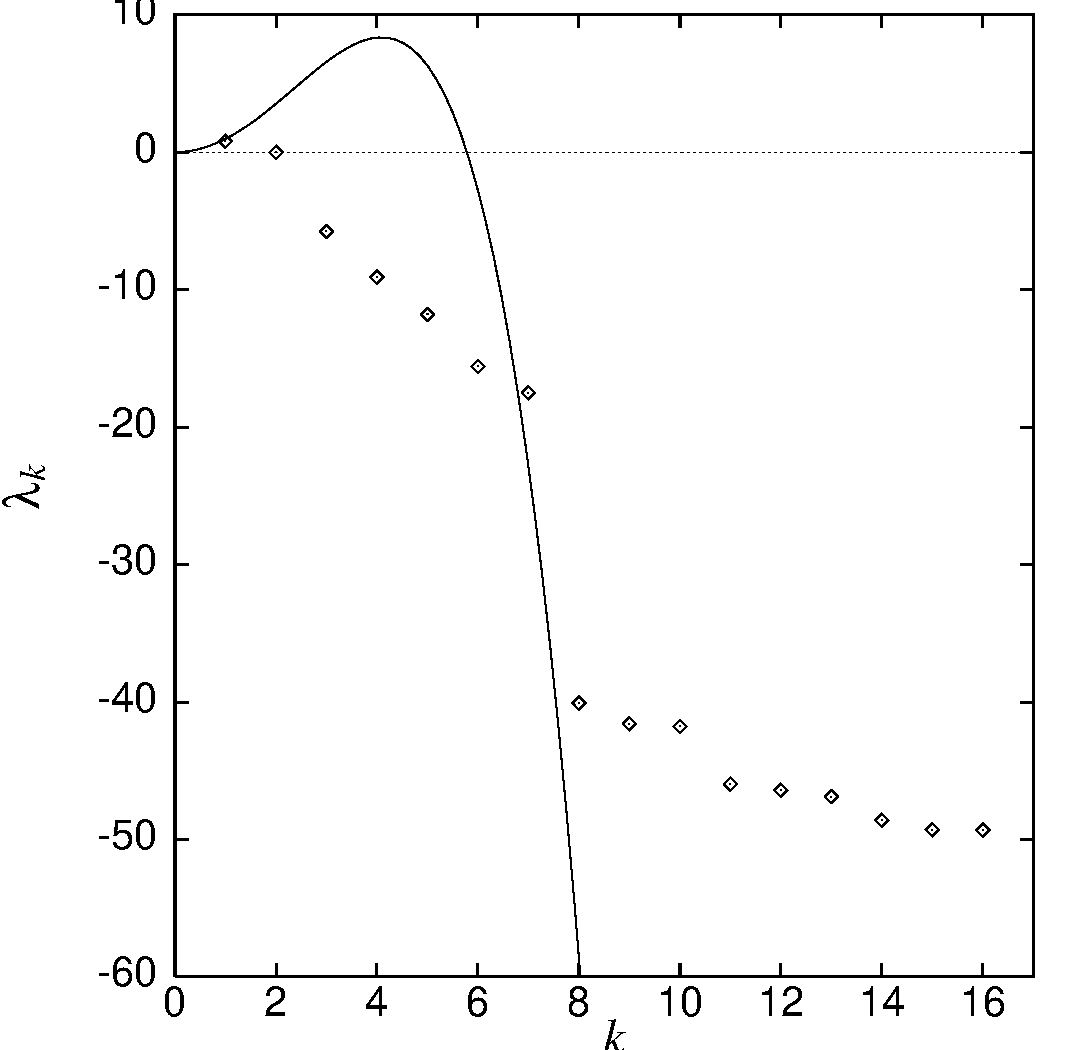
\includegraphics[width=0.40\textwidth]{eigenvalues}
 (b)~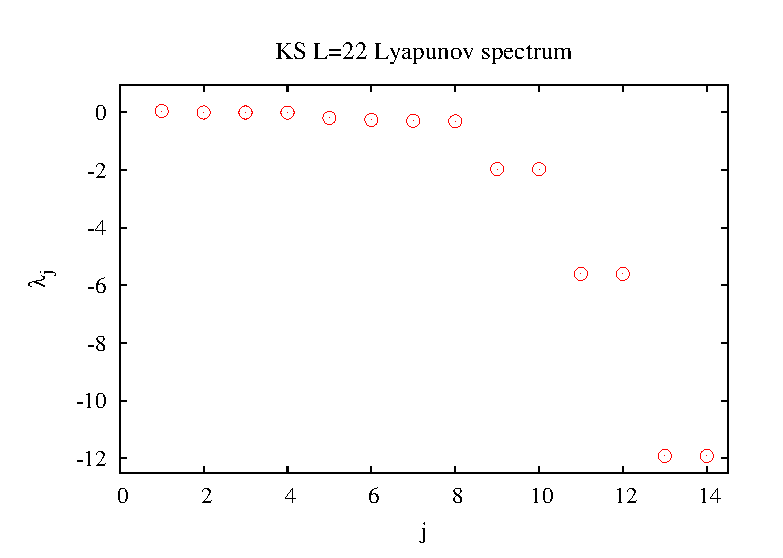
\includegraphics[width=0.50\textwidth]{lyapSpec}
\caption{
(a)
Lyapunov exponents $\lambda_k$ versus $k$ for the periodic
orbit $\overline{1}$ compared with  the stability eigenvalues
of the $u(x,t)=0$ stationary solution $k^2- \nu k^4$ (from
\refref{Christiansen97}). $\lambda_k$ for $k \geq 8$ fall
below the numerical accuracy of integration and are not
meaningful. Antisymmetric subspace,
hence no \SOn{2}\ pairing of eigenvalues, $N=16$ real Fourier
modes, $L=36.31$. One needs to rescale the time to compare
this to figure (b); -60 in the Lyapunov scale of figure (a)
corresponds to approx. -1.8 in figure (b).
(b)
First 14 Lyapunov exponents $\lambda_j$ for the full
\statesp, periodic b.c. KS for $L=22$, from a 62 real Fourier
modes long-time simulation (from \refref{SCD07}).
}
\label{fig:lyapSpec}
\end{figure}


\begin{description}
\item[2009-09-13 Predrag]
Sure looks persuasive, see \reffig{fig:lyapSpec}. I have also
added stability of a periodic orbit from
\refref{Christiansen97}, for KS on the periodic b.c.,
antisymmetric subspace, system size $\tilde{L} = 5.8$ close
to the onset of chaos, 16 real Fourier modes. As (perhaps?)
discussed in \refref{lanCvit07}, one has to be careful about
defining the effective system size $\tilde{L}$ for the
antisymmetric subspace, so these computations are done on
$L=36.31$ (or $L = 18.155$ if one considers the fundamental
$[0,L/2]$ domain only). Going from $(L,\nu) =
(2\pi,0.029924)$ of \refref{Christiansen97} to $(L,\nu) =
(L,1)$ convention used here requires that the time be
rescaled as $t \to \nu t$, and the Lyapunov exponents as
$\lambda_i \to \lambda_i/ \nu = \lambda_i/ 0.029924 $, so -60
in the Lyapunov scale of \reffig{fig:lyapSpec}\,(a)
corresponds to approx. -1.8 on the scale of
\reffig{fig:lyapSpec}\,(b), which would mean that then we
computed only the first pair of isolated eigenvalues. The
reason is that for periodic orbits we are computing {\em
Floquet multipliers} which underflow numerically very
quickly, so we cannot compute many {\em Floquet exponents}.
These covariant Lyapunov eigenvector methods are apparently
much smarter.

In \refref{lanCvit07} computations are done at $L = 38.5$,
but we listed only 4 eigenvalues per periodic orbit, and
considering hopeless organizational skills on the Lan astral
plane, I doubt that the full spectra can be rescued from
Lan's calculations. And, as explained above, probably we cannot
compute them for periodic orbits.

\item[Ruslan]
 Here's the expanded list of Lyapunov exponents for KS with $L = 22$:
 0.048,    0.0,    0.0,   -0.003,   -0.189,   -0.256,   -0.290,   -0.310,
-1.963,   -1.967,   -5.605,   -5.605,  -11.923,  -11.923...
So, there appears to be 8 `physically relevant' exponents and
the rest are pairs of hyperbolically separated ones.

I read
the papers about these covariant Lyapunov vectors and I'm not
sure I understand how they are related to eigenvectors at
periodic orbits: are they aligned?  I suspect that not quite,
apart from the most expanding and the most contracting
direction, the rest are sitting somewhere within the
subspaces spanned by the $k$ most expanding, or $m$ most
contracting eigendirections, but not quite aligned with the
eigendirections themselves.  That's probably why they are
more appropriately called `Lyapunov vectors'.

\item[2009-09-14 Predrag]
The `covariant Lyapunov vectors' are indeed the (right,
non-orthogonal) eigenvectors of the \jacobianM\ \jMps, as
defined in ChaosBook, and coincide with Floquet eigenvectors
for a periodic orbit.

 \item[Ruslan] I use 32 complex Fourier modes, so the
truncated system has 62 degrees of freedom.  The Lyapunov
exponent calculation is standard (using Gram-Schmidt).  The
exponents are the same, independent of the method of
calculation.  I have not attempted to calculate the covariant
Lyapunov vectors. I'm pretty sure that
orthogonality between physical and isolated eigenvectors
applies, but have not checked.

 \item[Ruslan]
It's OK to I email Hong-liu
Yang\rf{YaTaGiChRa08}, ask him to rerun his covariant
Lyapunov vector spectrum for $L=22$, to see whether he agrees
with us.

 \item[Ruslan]
I have the 62 eigenvalues/eigenvectors for all the RPO/PPO
I've detected, but for the highly contracting eigenvalues
the straightforward calculation
suffers from the numerical noise. We need a
better method to compute Floquet multipliers. I have now
checked:   Looks like {Kurt Lust} has proposed one, but I
cannot get his paper on ``Improved Numerical Floquet
Multipliers''\rf{Lust01}. If you could
get it for me, it would be great.

\item[2009-09-13 Ruslan]
``Structure of characteristic Lyapunov
vectors in spatiotemporal chaos''\rf{PaSzLoRo09} states
that characteristic Lyapunov vectors ``reduce to the Floquet
eigenvectors for a periodic orbit'' and references Trevisan
and Pancotti\rf{TrePan98}, which I cannot get electronically.

\item[2009-09-14 Predrag]
I added abstracts of these papers to the reading list above.
The `covariant Lyapunov vectors' are indeed the (right,
non-orthogonal) eigenvectors of the \jacobianM\ \jMps, as
defined in ChaosBook, and coincide with Floquet eigenvectors
for a periodic orbit. For a flow they are defined at a given
\statesp\ point by going back and forward a finite, but
`sufficiently long' time $t$, and coincide with the Floquet
eigenvectors if the point is (relative) periodic. I believed
that for a PDE we cannot go backward, but was wrong; the do
it by using the segment of forward trajectory stored in
memory. The reason why one can get the Floquet {\em exponent}
for arbitrarily long orbit is that the multiplier for eigenvector
evolved in time is just a number, so taking its logarithm over
short time segments and
storing it is trivial, no underflow problems one would get if
one worked with the Floquet {\em multiplier}. So we should be able
to keep track of all 62 eigenvectors, redo it for 126 eigenvectors,
and compare with plots in \refref{YaTaGiChRa08}.
Ginelli \etal\rf{ginelli-2007-99} are the main
reference on the `covariant Lyapunov vectors.' They describe
the QR algorithm for computing Gram-Schmidt vectors (GSV) and
recovering the covariant Lyapunov vectors (CLV) from them.
What confuses me is that so far all papers refer to $\Lyap_j
= \eigRe_j + i \, \eigIm_j$ as purely real, and list only
$\eigRe_j$, but I guess that will be explained somewhere.

\item[2009-09-14 Predrag]
My initial \reffig{fig:lyapSpec} was not optimal; I have now
reploted it as in Fig.~4 of
Yang \etal\rf{YaTaGiChRa08},
agrees with their 'extensivity' plot for $L=96$ and $192$.

I prefer $x$-axis to be $j/\tildeL = 2 \pi j/L$, as in
\reffig{fig:lyapSpecRscld}.

I do not like the way they count eigenvalues:  due to the $\On{2}$
2-dimensional irreducible representations
one should group their $j,j+1$ pairs,
plot them as a single, two-valued $j$, as in
\reffig{fig:lyapSpecRscld}. What one chooses to pair for low
$j$ might be ambiguous, as the nonlinear interactions mix up
the $\On{2}$ 2-dimensional linearly irreducible representations.
Reploted as in our much ignored 1997 paper\rf{Christiansen97},
eigenvalues fall onto $ (2 \pi j/L)^2 - (2 \pi j/L)^4 $
\eqv\ $\EQV{0}$  stability curve.
The isolated `covariant Lyapunov vectors'
are damped by $-(2 \pi j/L)^4$. I worry that we will not have such
amicable divorce for plane Couette and pipe flows...

% PC 2009-09-14: (b) generated by siminos/figSrc/gnu/lyapSpec.gnu
\begin{figure}
 (a)~\includegraphics[width=0.50\textwidth]{YaTaGiChRa08fig4}
 (b)~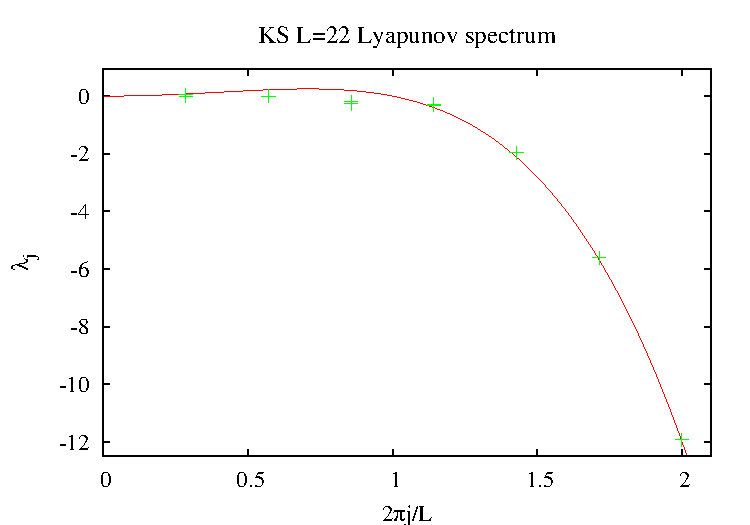
\includegraphics[width=0.40\textwidth]{lyapSpecRscld}
\caption{
(a)
Fig.~4 of
Yang \etal\rf{YaTaGiChRa08}:
Extensivity of the Lyapunov spectrum for the KS equation with
periodic b.c.. Inset: number of non-negative exponents (circles),
Kaplan-Yorke dimension (squares), metric entropy (diamonds,
multiplied by $50$), and number of physical modes (triangles).
In perfect agreement with
\reffig{fig:lyapSpec}\,(b) here, plotted the same
(incorrect) way.
(b)
First 14 Lyapunov exponents $\lambda_j$ for the full
\statesp, periodic b.c. KS for $L=22$, from a 62 real Fourier
modes long-time simulation (from \refref{SCD07}).
The same as in part (a) and in \reffig{fig:lyapSpec}\,(b), but
abscisa is $j/\tildeL = 2 \pi j/L$, and each $j$ labels
the $\On{2}$ 2-dimensional irreducible representation
Lyapunov exponents pair.  Full line corresponds to
the stability eigenvalues
of the $u(x,t)=0$ stationary solution
$(j/\tildeL)^2- (j/\tildeL)^4$, for arbitrary system size $L$.
}
\label{fig:lyapSpecRscld}
\end{figure}


We also see
that the `physical' modes are split into a less contracting 1/2
and more contracting 1/2 (different slopes in the
\reffig{fig:lyapSpecRscld}\,(a)). We
used to think the first 1/2 is the physically important one,
and say so in the arXiv version 2 of the article.
We stand corrected.

The Floquet eigenvectors of our (relative) periodic orbits are
what they call 'covariant,' so they should fit into their finite back/forth
time vectors like into a glove, whenever the respective state space
points are sufficiently close.

The main point of exploring the ergodic states space hierarchically
by periodic orbits is to tessellate it systematically, in the most
uniform way, by neighborhoods (linearized stable/unstable manifolds)
of periodic points. A periodic solution computed on a small system
size $L$, periodic b.c. is a solution on any multiple of $L$, and it comes
together with a smooth family of corresponding solutions for nearby
$L$'s.

I see prospects of a long and happy marriage here.

\item[2011-02-04 ES] Talked to Hugues Chat\'{e} and Kazumasa Takeuchi.
I was at CEA/Saclay for a thesis presentation today, bumped into Chat\'{e}
and
\HREF{http://daisy.phys.s.u-tokyo.ac.jp/student/kazumasa/}{Kaz}
(actually, it was more like invading their offices). Kaz updated me on
their latest work on Lyapunov vectors. We finally all agreed that we would give
the periodic orbit - Lyapunov vectors project a second try and arrange to meet
in Paris. I'll keep you posted.


\item[2011-02-07 ES] Sent Kaz an initial condition for a KS, $L=22$ \po\
with $T_p=10.2534$.

\item[2011-02-09 Kaz] I tried your initial condition and it works perfectly!
I also tried to calculate the Lyapunov exponents associated to this UPO.
The largest is about 0.03328, right? I'm not yet really sure about this value,
so it would be nice if you let me know the Lyapunov exponents you know for this UPO.

\item[2011-02-11 ES] The Lyapunov exponent I have is 0.033163, so you
are pretty close. In fact this exponent has multiplicity two, and
there is no other positive exponent for this orbit.

\item[2011-02-11 Kaz] Great! All you are saying (multiplicity, only two positive
exponents) are exactly what I confirmed with that UPO. I will soon have all
the necessary information regarding the physical/spurious modes for that UPO.

\item[2011-02-11 Kaz] Which quantities/properties do you have
analytically/numerically for these UPOs in your methods? For instance,
if we know the time evolution operator for a UPO, we can compute both
Lyapunov exponents and covariant Lyapunov vectors as eigenvalues and
eigenvectors of that operator. Do you have them? Or, the exponent values
you have are just computed by Bennetin's standard algorithm?

\item[2011-02-11 ES] We do not use Bennetin's method, but rather
something similar to what you just described. However, I am not sure how
you exactly define the time evolution operator, so I will describe with
details what we do.

Given an initial condition $x_o$ and period $T$ for a UPO, we integrate
for $t=0$ to $T$, the differential equations for the nonlinear flow
$dx/dt=v(x)$, and a differential equation for the Jacobian matrix:
$dJ(t,x_o)/dt = A(x)J(t,x_o)$, with initial condition $J(0,x_o)=1$.
Here $A_{ij}(x)=\partial v_i/\partial x_j$. The eigenvalues $\Lambda_i$ of $J(T,x_o)$ are
the Floquet multipliers and its eigenvectors the Floquet eigenvectors
(the covariant Lyapunov vectors for UPOs). Then the i'th Lyapunov exponent is
$\mu_i = \ln(|\Lambda_i|)/ T$
(for periodic orbits we usually call them Floquet exponents).
Although we only have the eigenvalues in file, I could easily compute
the eigenvectors for comparison.

The problem with this approach is that, while we believe the leading
eigenvalues to be accurate, the highly contracting ones suffer from
numerical noise. So it would be hard for us to separate physical from
isolated eigenvectors based on this computation alone.

\item[2011-02-11 Kaz] Thank you for the explanation. That is exactly what
I meant by eigenvalues of the time evolution operator.

Myself, I compute the Lyapunov exponents (and the covariant vectors) simply
by Benettin's method (and by Ginelli's one). The only trick is that, each time
the trajectory x(t) returns to its original position x(0), i.e., at every cycle
of the orbit, I replace x(t) by its initial value x(0). This is to kill
numerical noise that would grow and eventually kick the trajectory
out of the periodic orbit. This method is accurate even for very small
exponent values.

\item[2011-02-20 Predrag] to Kaz:

I'm very glad that you and Evangelos are looking at the KS periodic solutions.
Attached is \refsect{sect:LyapKS} from out blog
(you probably have this already, but
I am not quite sure) - if you plot all cycle Floquet multipliers, can you try to
also plot them in the way suggested in my notes (it differs a bit from how you
had plotted them in Yang \etal\ paper\rf{YaTaGiChRa08})?
I was pleasantly surprised how well one
could see the physical/isolated boundary already for $L=22$.


\BFIG{1.0}   % width=#1\textwidth
{kaz2-PhysModes}   % f_name.pdf
{}   % short caption text
{    % full caption text
kaz2-PhysModes
}
{kaz2-PhysModes}   % f-figure-label

\BFIG{1.0}   % width=#1\textwidth
{kaz4-VectCompar}   % f_name.pdf
{}   % short caption text
{    % full caption text
kaz4-VectCompar
}
{kaz4-VectCompar}   % f-figure-label

\BFIG{1.0}   % width=#1\textwidth
{kaz5-AngleTimeSeries}   % f_name.pdf
{}   % short caption text
{    % full caption text
kaz5-AngleTimeSeries
}
{kaz5-AngleTimeSeries}   % f-figure-label

\SFIG{kazUPOa}   % width=#1\textwidth
{}   % short caption text
{    % full caption text
kazUPOa
}
{kazUPOa}   % f-figure-label

\item[2011-02-21 Kaz]
I (with spirits of Hugues Chat\'e and Francesco Ginelli hovering above me)
have integrated some of
them and computed a number of quantities to elucidate the
physical/isolated separation of Lyapunov modes. Here I show you a
summary of preliminary results. I also have some questions to ask you
(see the end of the mail for them).


\textbf{Results}

Here we concentrate on (1) a chaotic trajectory generated from a random
initial condition, and (2) the first periodic orbit in the list
Evangelos sent to me ($T=10.25336729174627$; called "UPOa" in the attached
figures). The numerical integration of the {unstable \po} is done by replacing the
trajectory on each period by the initial condition of the {unstable \po}.

First, the top two figures in fig2...pdf show the Lyapunov spectrum for
the trajectory (1) and the {unstable \po} (2). For the {unstable \po} the exponents are simply
given by the Floquet multipliers, as indeed confirmed quantitatively,
while for the trajectory they are of course different, though close,
from those of the {unstable \po} (top right figure). Increasing the index, we can
see the appearance of the step-wise structure (top left figure) like in
our PRL paper.

The bottom two figures show the hyperbolic isolation of the physical and
isolated modes (similar to Fig.2(d,e) in our PRL; I remind you that we
CANNOT define them solely from the Lyapunov exponents.). The quality of
the data is not satisfactory because of the present length of the
simulation, but we can see that there are at most 11 physical modes.


fig4...pdf compares the structure of Lyapunov vectors (always covariant
in this mail) between the trajectory and the {unstable \po}. I monitored the
chaotic trajectory and used the moment when it gets closest to the {unstable \po}
during the simulation. The inset of the top left figure shows the
snapshot of the trajectory (blue) and the {unstable \po} (red) at that moment.

The other three subpanels compare the vector structure at the same
moment. Here the spatial shift between blue and red is already taken
into account, so that you can directly compare the two profiles. The
bottom two figures show the 6th and 9th modes, which correspond to
real-valued Floquet multipliers of the {unstable \po} (thus Oseledec subspace is
not degenerated). We can see that the vectors of the chaotic trajectory
become quite close to the {unstable \po} counterparts (but not exactly; some are
better, others are not as good). For the Lyapunov modes that correspond
to complex conjugate pairs of the Floquet multipliers, e.g. 1st and 2nd
ones, we have to compare a vector of the trajectory with arbitrary
linear combinations of the 1st and 2nd {unstable \po} vectors. Indeed, we can find
a combination that gives a structure similar to the vector of the
trajectory.

In short, as a chaotic trajectory wanders among {unstable \po}s, the vectors of the
trajectory change their shape incessantly to follow the vectors of the
closest {unstable \po} at each moment.


Now, the question is whether we can unambiguously define the physical
and isolated modes for each periodic orbit, or not. We don't know how to
do this for the moment, because the angle between any Lyapunov vectors
of {unstable \po} varies periodically and thus does not reach 0 or pi forever.

Moreover, we find that the hyperbolicity properties crucially depend on
the quality of the periodic orbit. See fig5...pdf, which shows
time-series of angles between given pairs of the Lyapunov vectors of the
{unstable \po}. Although the angle between Lyapunov modes of index >=11 (correspond
to isolated modes for the chaotic trajectory) stays close to pi/2 with a
seemingly trivial time-evolution, the numerically computed angle is not
strictly pi/2 and is subject to a very slow convergence (see the middle
panel). To test, I added a noise to the initial condition of the {unstable \po} and
computed the same quantities. While the angles for index $\leq 10$ do not
show significant changes, those for index $\geq 11$ show spurious
oscillations with long periods.

This is why we think that the quality of the periodic orbit is crucial.
It could be that, if we had an initial condition with infinite
precision, the angle for index $\geq 11$ are strictly orthogonal, and thus we
could define the isolated modes from this strict orthogonality.


\textbf{Questions}

1) We wonder if we may define the physical and isolated modes for
periodic orbits. Do you have any ideas, in particular from the viewpoint
of the Floquet multipliers and eigenvectors? If the isolated modes of
{unstable \po}s are strictly orthogonal, it means that the Jacobian matrix for a
cycle can be decomposed to two parts, one of which would be an
orthogonal submatrix. Is it likely to you?

2) As shown above, the quality of the {unstable \po} initial conditions turns out
to be crucial. Do you have data with better resolutions? Or, is it
numerically difficult to compute {unstable \po}s with very high resolutions?

That's all for now. Any comments / questions are of course welcome!


\textbf{Kaz to Predrag} I made a plot of the Lyapunov spectrum of
the {unstable \po} (the same one as above) in the same way as you did. See UPOa.pdf
and UPOa-lyap.dat. I hope this is the one you wanted.

                            \noindent
 3.3274529258200000e-2    \\
 3.3273022876699997e-2    \\
 1.2294744377000001e-5    \\
 -1.3236540275600000e-5    \\
 -7.2634814842399998e-5    \\
 -2.1629227416399999e-1    \\
 -2.6517234146000002e-1    \\
 -2.6516527982799998e-1    \\
 -3.3072168309500000e-1    \\
 -1.9602739059100001    \\
 -1.9673554279600001    \\
 -5.6025023421000002    \\
 -5.6042396292200003    \\
 -1.1925106699200001e+1    \\
 -1.1925523679299999e+1    \\
 -2.2011597078699999e+1    \\
 -2.2011657848500001e+1    \\
 -3.7116197744200001e+1    \\
 -3.7116202659300001e+1    \\
 -5.8760926784699997e+1    \\
 -5.8760926787599999e+1    \\
 -8.8935807811399997e+1    \\
 -8.8935807884699997e+1    \\

\end{description}
